\documentclass[a4paper,14pt]{extarticle}
\usepackage{array,amsmath,fancybox,amsfonts,graphicx,amsthm,amssymb,wasysym,latexsym,slashed,anysize,subfigure,calc}
\usepackage[spanish]{babel}
\usepackage[utf8]{inputenc}
\usepackage{fancyhdr,float,hyperref}
\usepackage{lettrine}

\usepackage{enumitem}


%fractiones grandes en inline text: inventa un comando \ddfrac
\newcommand\ddfrac[2]{\frac{\displaystyle #1}{\displaystyle #2}}

%lewis y química
\usepackage{chemformula,elements}
%chemformula, provides \ch{} with the !(<below>)(<formula>) syntax and \chlewis;
%elements, provides \elconf and \writeelconf.
%ex:
%\ch{
%  !(\elconf{Li})( "\chlewis{180.}{Li}" ) +
%  !(\elconf{F})( "\chlewis{0.90:180:270:}{F}" )
%   ->
%  !(\writeelconf{2})( Li+ ) +
%  !(\writeelconf{2,2+6})( "\chlewis{0:90:180:270:}{F}" {}- )
%}


%entorno para química: texto y math mode
%\newcommand*\chem[1]{\textup{#1}}
\newcommand*\chem[1]{\ensuremath{\mathrm{#1}}}

%column
\usepackage{multicol}
%uso: \begin{multicols}{3}

%enumitem: configurar listas
\usepackage{enumitem}

%para los entornos de soluciones
\usepackage{mdframed,xcolor,color}
	%uso: 	entorno (begin,end): {mdframed}[backgroundcolor=brown!10] 

%subrayado y highlight. Tiene que estar detrás de usepackage[color]
\usepackage{soul}
	%\textst{normal} 
	\DeclareRobustCommand{\hlcyan}[1]{{\sethlcolor{cyan}\hl{#1}}} %en cyan!
		%\hl{highlighted text} %uso


%tamaños fuentes extra: 8,9,14,17,20
	\usepackage{extsizes}
	
 	%fuente librebaskerville
 	\usepackage[T1]{fontenc}
	\usepackage{librebaskerville}
	
	%fracciones $$ en texto más elaboradas
	 \usepackage{xfrac}
	 
	%permitir que una ecuación larga esté separada por un salto de página
	\allowdisplaybreaks[4]
		
	%gráficos varios 
	\usepackage{graphics}
	
	%fancy tables
	\usepackage{booktabs}
	\usepackage[small,centerlast,up]{caption}

	
	%mejora en la exposición de guarismos
	\usepackage{numprint}
	
\usepackage{everypage,draftwatermark} %Marca de agua
\SetWatermarkText{\vspace*{2cm}

\hspace*{2cm}\parbox{2\textwidth}{\centering DIST.\\B1-FyQ}}
\SetWatermarkScale{1.5}
\SetWatermarkLightness{0.9}

\DeclareMathOperator{\lin}{lin}
\DeclareMathOperator{\id}{\textbf{id}}
\DeclareMathOperator{\modulo}{mod}

\newcommand{\mc}[3]{\multicolumn{#1}{#2}{#3}}
\newcommand{\halmos}{
\vspace*{-4ex}

\begin{flushright}
\rule{1mm}{2.5mm} \end{flushright}
\vspace*{-3.5ex}

}
\renewcommand{\qed}{\halmos}


%versores: %uso: \uveci\ne\hat{\imath}_{\uvec{i}}+\uvec{j}+\uvec{k}$
\usepackage{bm}
\newcommand{\uveci}{{\bm{\hat{\textnormal{\bfseries\i}}}}}
\newcommand{\uvecj}{{\bm{\hat{\textnormal{\bfseries\j}}}}}
\DeclareRobustCommand{\uvec}[1]{{%
  \ifcsname uvec#1\endcsname
     \csname uvec#1\endcsname
   \else
    \bm{\hat{\mathbf{#1}}}%
   \fi
}}


%algún nuevo operador
\DeclareMathOperator{\cotan}{cotan}


%para textbf en entorno enumerate
\renewcommand{\labelenumi}{%
 \textbf{\theenumi}.
}

%a4
\marginsize{.5cm}{1cm}{1cm}{1cm}%requiere el paquete anysize,izq,dcha,arriba,abajo

%a5
%\marginsize{1cm}{1cm}{1cm}{.5cm}%requiere el paquete anysize,izq,dcha,arriba,abajo

\newtheorem{teo}{{\sc \textbf{Teorema}}}
\newtheorem{defi}{{\sc \textbf{Definición}}}
\newtheorem{coro}{{\sc \textbf{Corolario}}}


%opening
\title{\textbf{	}}
\date{}
\pagestyle{fancy}
\fancyhead[LO,RE]{{\small DOSSIER DE PROBLEMAS\hspace{1ex} \textbf{2Ev}}}
\fancyhead[RO,LE]{{\small B1-DIST\hspace{2ex} FÍSICA y QUÍMICA}}
%\fancyhead[CO,CE]{Ricardo Torres\\http://tinyurl.com/iesCMGfyq}



\begin{document}
\pagenumbering{gobble}

%gas ideal y mezclas
%disoluciones
%estequiometría: ajuste, reactivo limitante, reactivos en disolución e impuros


\begin{enumerate}
  \setlength\itemsep{1.5em}
    
    
    \item (1 punto) Asumiendo que los gases de los que se habla en los siguiente enunciados pueden aproximarse como gases ideales:
    	\begin{itemize}
    		\item[a)] Calcula \textit{razonadamente} la presión parcial de $\chem{NO_2}$, medida en $mmHg$, en $50$ moles de una mezcla gaseosa equimolar de hexafluoruro de azufre y dióxido de nitrógeno en condiciones normales de presión y temperatura. 
    		%380 Torr
    		\item[b)] Dos gases puros, \textit{viz.}: metano y hexafluoruro de azufre, se guardan en sendas ampollas. \textit{Razona} cuál de los dos tendrá más densidad en condiciones estándar de presión y temperatura.
    		%Es más denso el hexafluoruro de azufre
    	\end{itemize}
    \qed
    
    
    \item (2 puntos) Un recipiente de $20\;mL$ contiene nitrógeno molecular a $25^\circ C$ y $0.8\;atm$; otro de $50\;mL$ contiene helio a la misma temperatura y a una presión de $0.4\;atm$. Tras conectar los dos recipientes a través de un pequeño tubo de volumen despreciable, y considerando ambos gases como ideales, estima \textit{razonadamente}:
    	\begin{itemize}
    		\item[a)] El volumen ocupado por cada gas y las presiones parciales de cada componente.
    		%el volumen es el mismo e igual al total disponible; pN2~0,23 atm; pHe=0,29 atm
    		\item[b)] La molaridad y el porcentaje en masa de $\chem{He}$ en la disolución.
    		%[He]~1.2E-2 mol/L; %He~15%
    		
    	\end{itemize}
	\qed   
	
	\item (1 punto) Responde \textit{razonadamente} a las siguientes cuestiones:
		\begin{itemize}
			%\item[a)] ¿Qué volumen debes tomar de una disolución $3\,M$ de ácido nítrico para preparar $500\;cm^3$ de otra que sea $2\,M$ del mismo ácido?
			\item[a)] La etiqueta de una botella de ácido clorhídrico comercial indica una concentración $15.5\,M$ y densidad $1.41\;g\,cm^{-3}$. Calcula su concentración como porcentaje en masa.
			%40,1%
			\item[b)] Se prepara una disolución con $3\;g$ de $\chem{KCl}$ y $200\;cm^3$ de agua de modo tal que la mezcla resultante tiene una densidad aproximada de $1.02\;g\,cm^{-3}$. Estima su concentración como porcentaje en masa.
			% ~1.5%
		\end{itemize}
    \qed
    
    
    
    
    \item (2 puntos)
    	\begin{itemize}
    		\item[a)] Considera la combustión de gas metano en condiciones normales. \textit{Razona} qué volumen de oxígeno molecular se requiere para quemar completamente $150\;L$ de metano.
    		%300 L
    		\item[b)] Se ponen a reaccionar $100\;g$ de cloruro de bario con $115\;g$ de sulfato de sodio para dar cloruro de sodio y sulfato de bario. Determina \textit{razonadamente} los gramos de sal común que resultan.
    		%56.5 g
    	\end{itemize}
    \qed
    
    \item (3 puntos) En un laboratorio a $50^\circ\,C$ y $3$ atmósferas de presión se hacen reaccionar $50\;g$ de un mineral de cobre de $90\%$ de pureza con $400\;mL$ de una solución $6\,M$ de ácido nítrico. Sabiendo que el rendimiento para la formación de dióxido de nitrógeno gaseoso es del $95\%$ y que se forma, además, nitrato de cobre{\small (II)} y agua,:
    	\begin{enumerate}[label=\alph*)]
    		\item Escribe y ajusta la reacción.
    		\item Identifica \textit{razonadamente }el reactivo limitante y calcula la masa que sobra del reactivo en exceso.
    		%6.6 g
    		\item Suponiendo que se comporta idealmente, calcula \textit{razonadamente} el volumen de dióxido de nitrógeno que se obtiene.
    		%10 L
    	\end{enumerate}
  	\qed
  	
  	
  	\item (1 punto) Resuelve \textit{razonadamente} las siguientes cuestiones: 
    	\begin{itemize}
    		\item[a)] El volumen molar, $\bar{v}$, de un gas se define como el volumen que ocupa un mol de gas.   		Calcula en condiciones normales el volumen molar de las siguientes especies gaseosas ideales:  \textit{	i) cloro molecular,\hspace{1ex}ii)  dióxido de azufre; y iii)	    una mezcla equimolar de cloro molecular y dióxido de azufre.}
    		\vspace{2ex}
    		
    		\item[b)] Para caracterizar cómo de bien se ajusta un gas \textit{real} al comportamiento ideal puede utilizarse el llamado \textit{factor de compresibilidad}, $Z$, que se define a través de la expresión $Z\equiv\dfrac{P\,\bar{v}}{RT}.$
    		%		con $\bar{v}$ el volumen molar, definido en el apartado anterior. 
    		
    		\vspace{1ex}
    		
    		Cuanto más difiera esta cantidad del valor que toma el factor de compresibilidad en el caso ideal, mayor será la desviación y menos preciso será utilizar la ecuación del gas ideal. ¿Cuál es el valor del factor de compresibilidad de un gas ideal?
    		
    		
    		
    		\begin{minipage}{.4\textwidth}
			\item[c)]  En la gráfica de la derecha se muestra el factor de compresibilidad en función de la presión para distintos gases \textit{reales} a una temperatura de $273\;K$. \textit{Razona} qué gas se acerca más al comportamiento ideal cuando está sometido a una presión de $400\;atm$.	
				%\vspace*{.2cm}
			\end{minipage}\hfill
	\begin{minipage}{.45\textwidth}
		\centering
		\vspace*{4ex}
		
		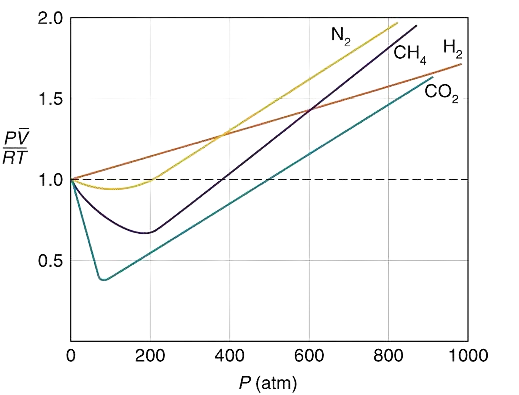
\includegraphics[scale=.5]{nitro.png}
	\end{minipage}			
    	\end{itemize}
    \qed 
\end{enumerate}

\end{document}

